\begin{center}
\footnotesize\noindent\fbox{
	\parbox{\textwidth}{
	Utilizzare le function degli Esercizi 4.1 e 4.6 per graficare l'approssimazione della funzione di Runge sull'intervallo \([-6, 6]\), per \(n = 2, 4, 6, \ldots, 40\). \\ \\Stimare numericamente l'errore commesso in funzione del grado \textit{n} del polinomio interpolante.
	}
}\end{center}

\noindent Di seguito i grafici che mostrano i polinomi interpolanti di grado \textit{n} calcolati usando come punti di interpolazione quelli corrispondenti alle \textit{n} ascisse di Chebyshev (evidenziati in rosso), sovraimposti al grafico della funzione di Runge \(f(x) = \frac{1}{1+x^2}\) (in blu). \\

\noindent\small\begin{tabular}{l*{5}{c}}
\hspace{3.5cm}\(n=2\) & \(n=4\) \\
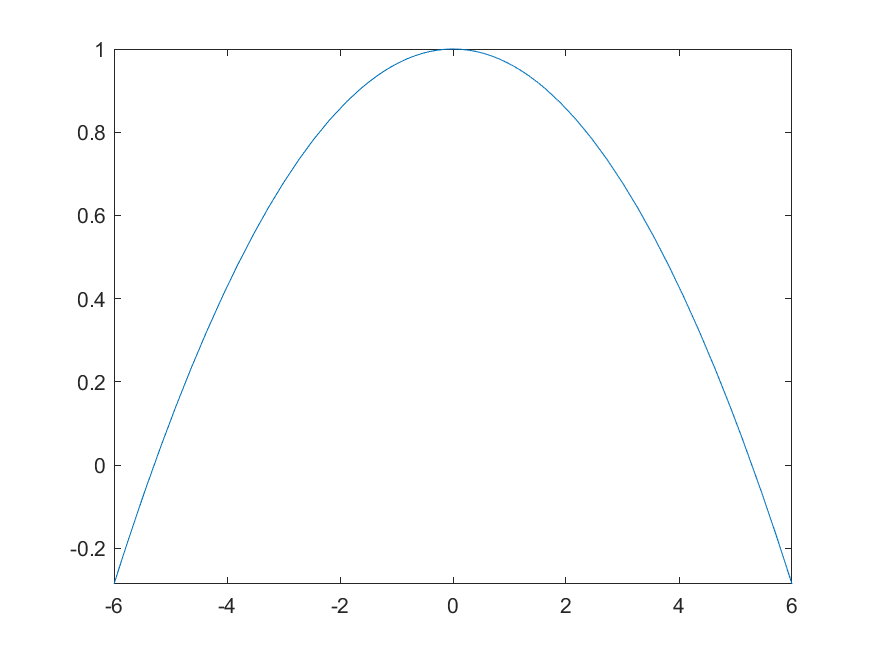
\includegraphics[scale=0.5]{cap4/4_7/2.png} &  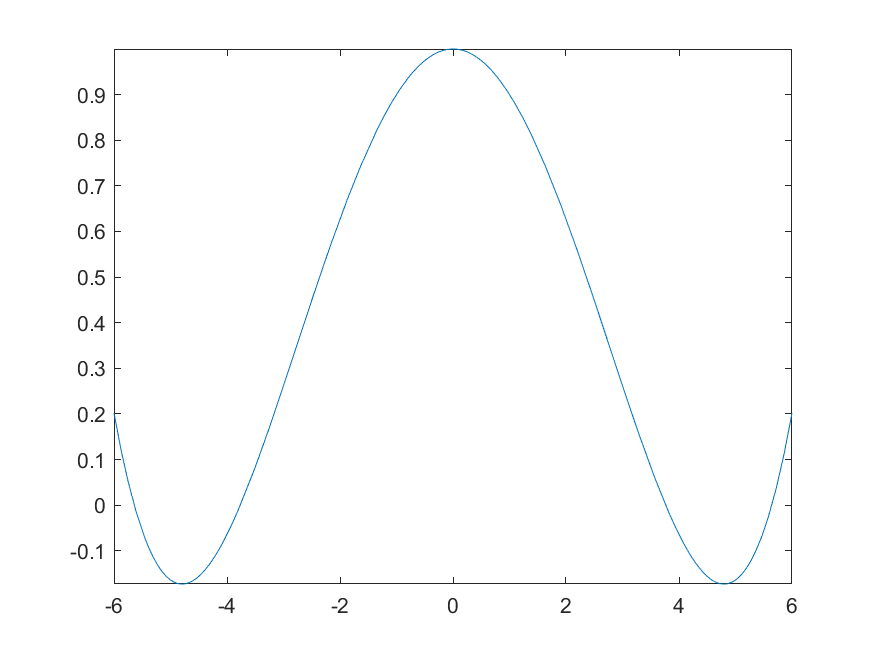
\includegraphics[scale=0.5]{cap4/4_7/4.png} \\

\hspace{3.5cm}\(n=6\)& \(n=8\) \\
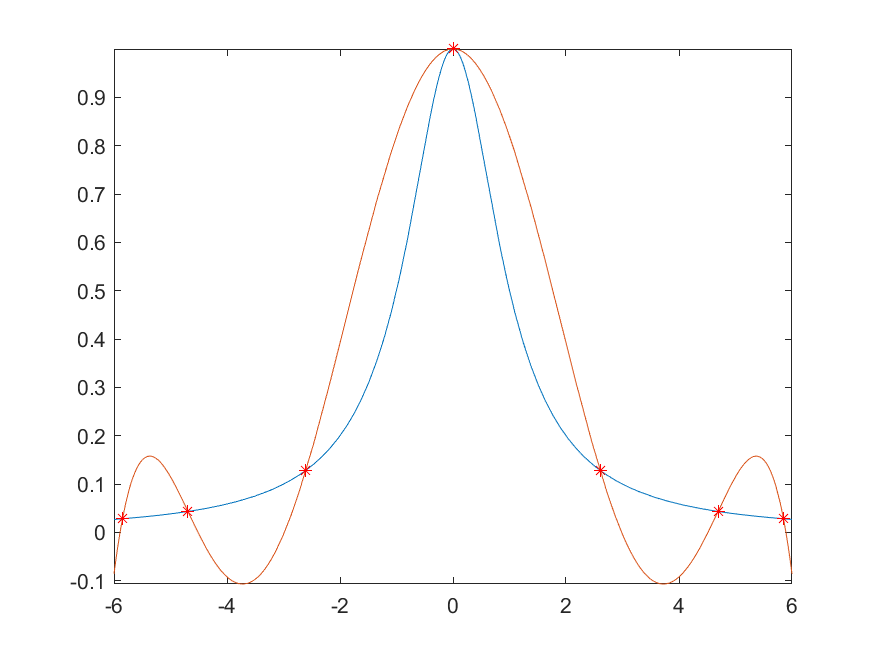
\includegraphics[scale=0.5]{cap4/4_7/6.png} &  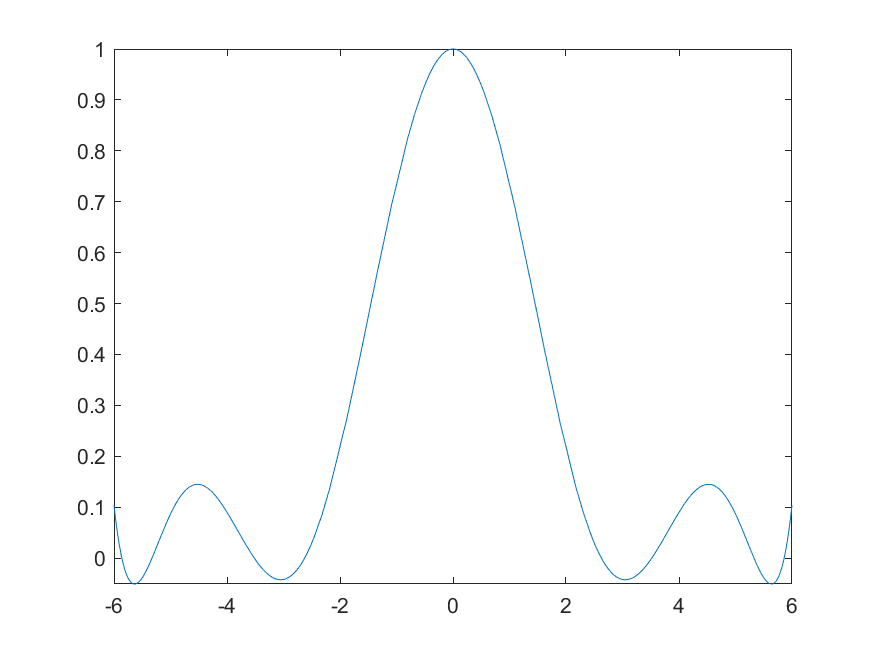
\includegraphics[scale=0.5]{cap4/4_7/8.png} \\

\hspace{3.5cm}\(n=10\) &  \(n=12\) \\
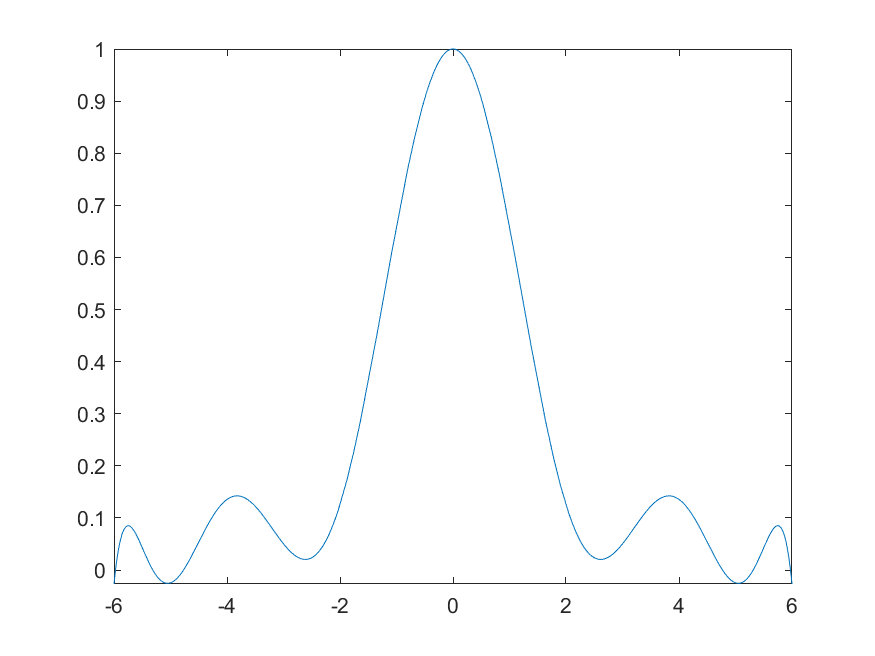
\includegraphics[scale=0.5]{cap4/4_7/10.png} &  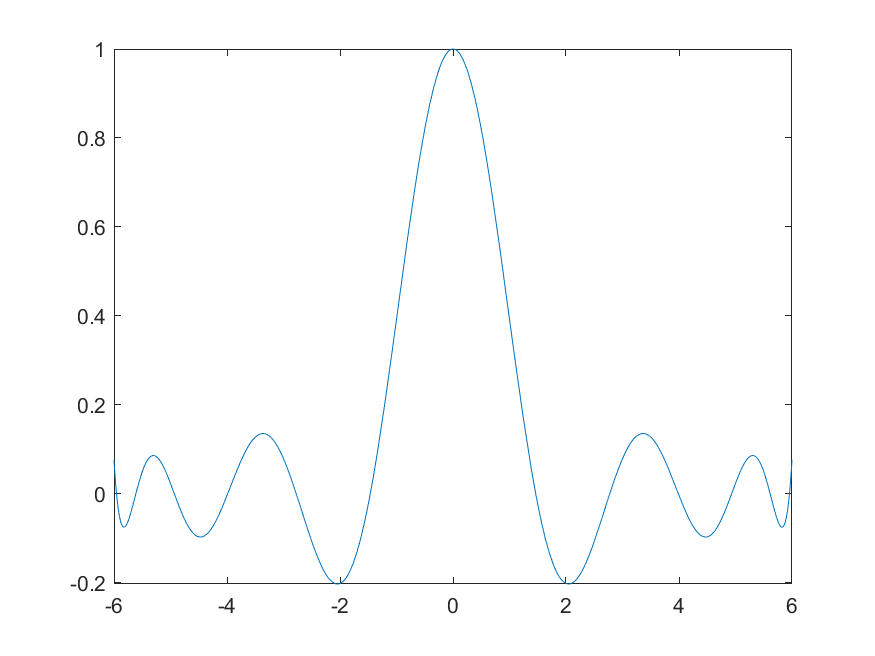
\includegraphics[scale=0.5]{cap4/4_7/12.png} \\
\end{tabular} \\ \\

\small\begin{tabular}{l*{5}{c}}
\hspace{3.5cm}\(n=14\) &  \(n=16\) \\
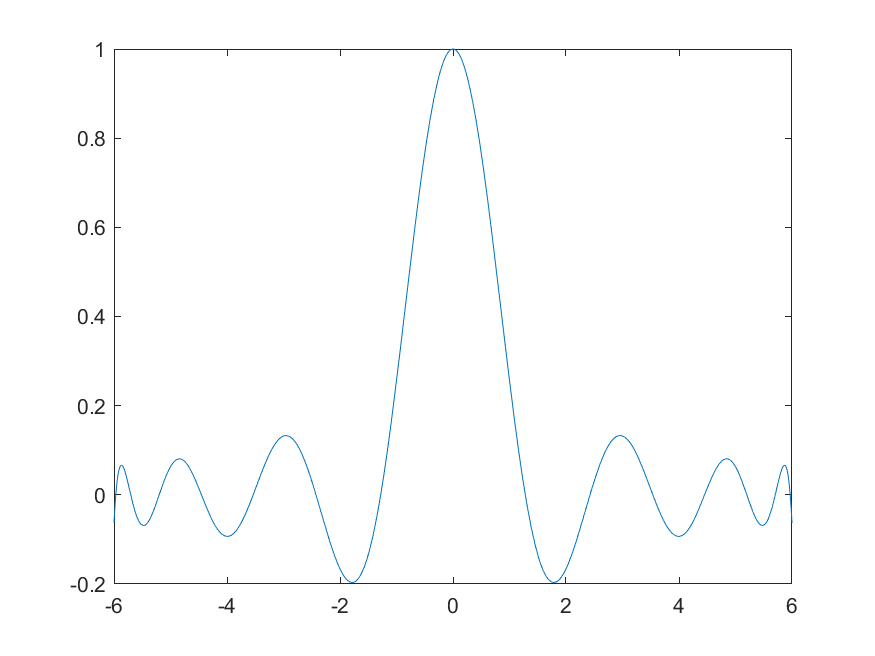
\includegraphics[scale=0.5]{cap4/4_7/14.png} &  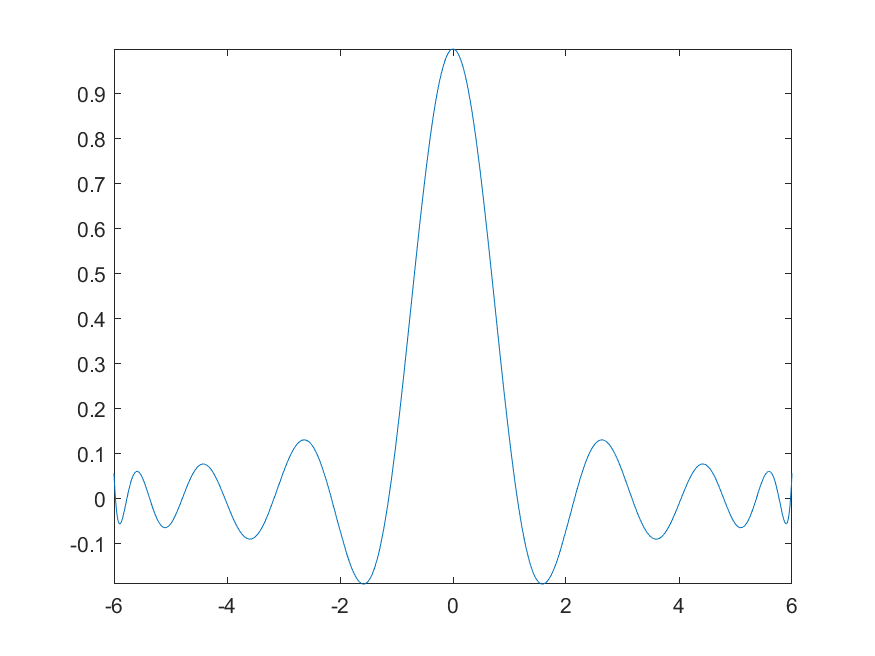
\includegraphics[scale=0.5]{cap4/4_7/16.png} \\

\hspace{3.5cm}\(n=18\) &  \(n=20\) \\
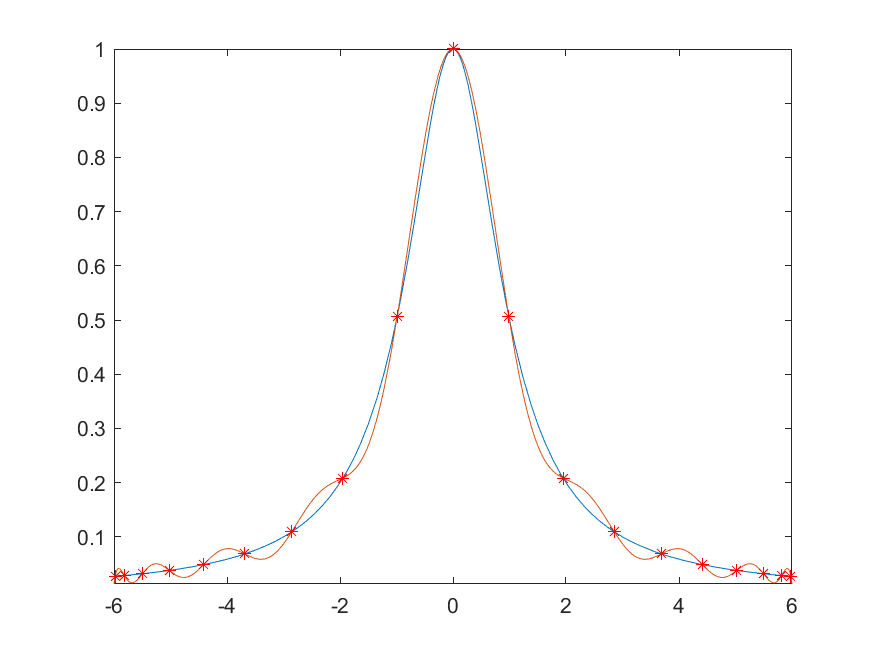
\includegraphics[scale=0.5]{cap4/4_7/18.png} &  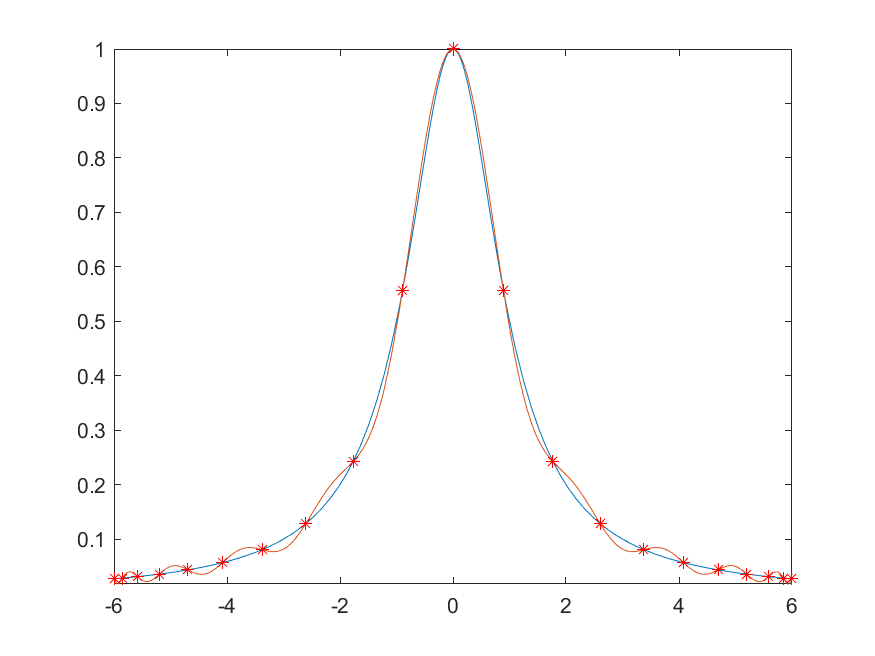
\includegraphics[scale=0.5]{cap4/4_7/20.png} \\

\hspace{3.5cm}\(n=22\) &  \(n=24\) \\
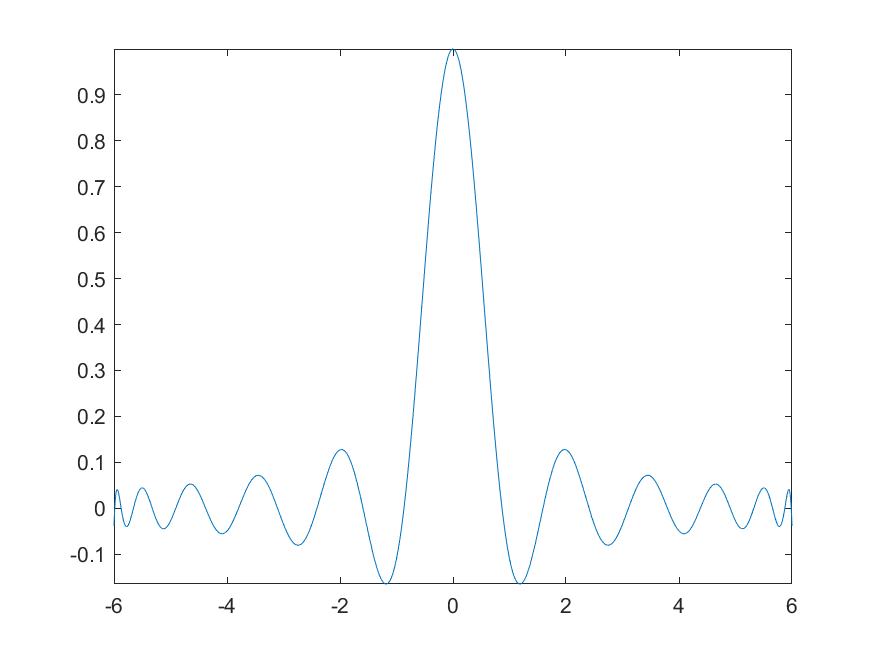
\includegraphics[scale=0.5]{cap4/4_7/22.png} &  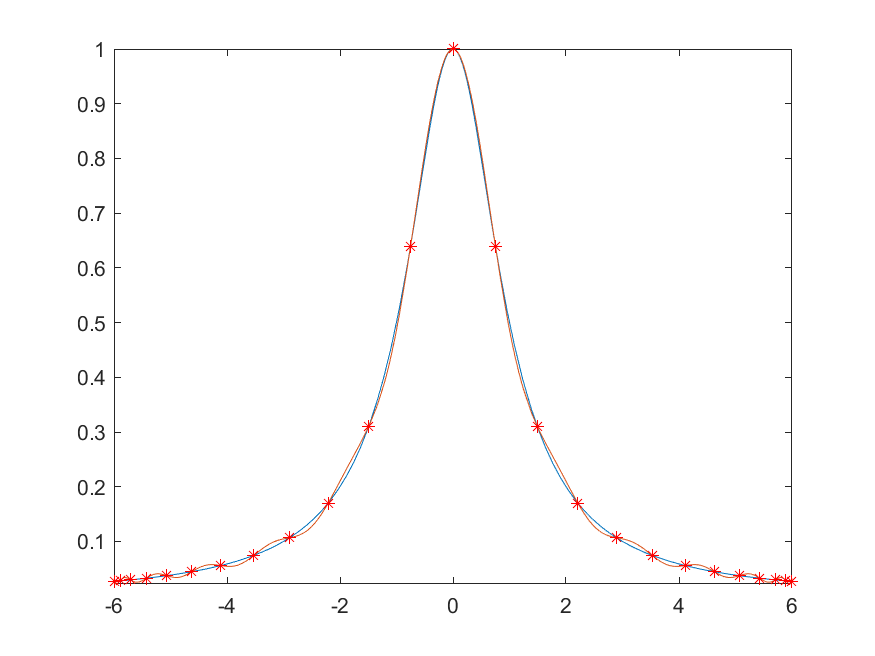
\includegraphics[scale=0.5]{cap4/4_7/24.png} \\

\hspace{3.5cm}\(n=26\) &  \(n=28\) \\
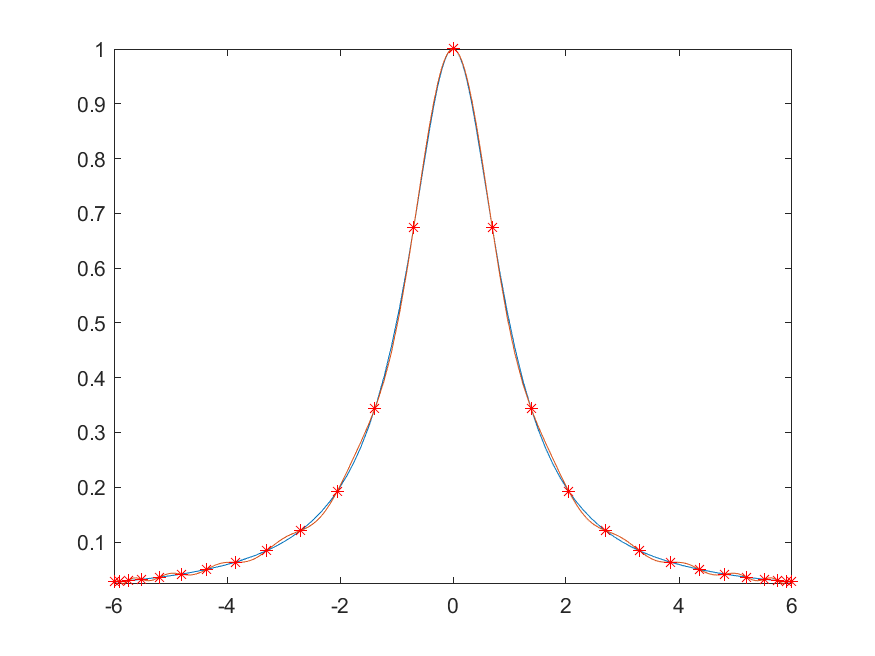
\includegraphics[scale=0.5]{cap4/4_7/26.png} &  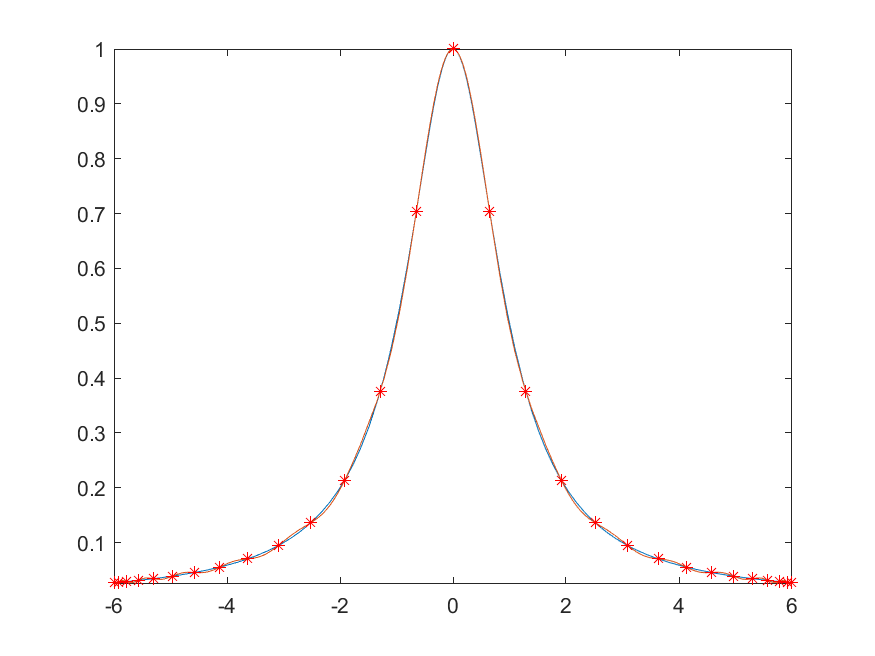
\includegraphics[scale=0.5]{cap4/4_7/28.png} \\
\end{tabular}

\small\begin{tabular}{l*{5}{c}}
\hspace{3.5cm}\(n=30\) &  \(n=32\) \\
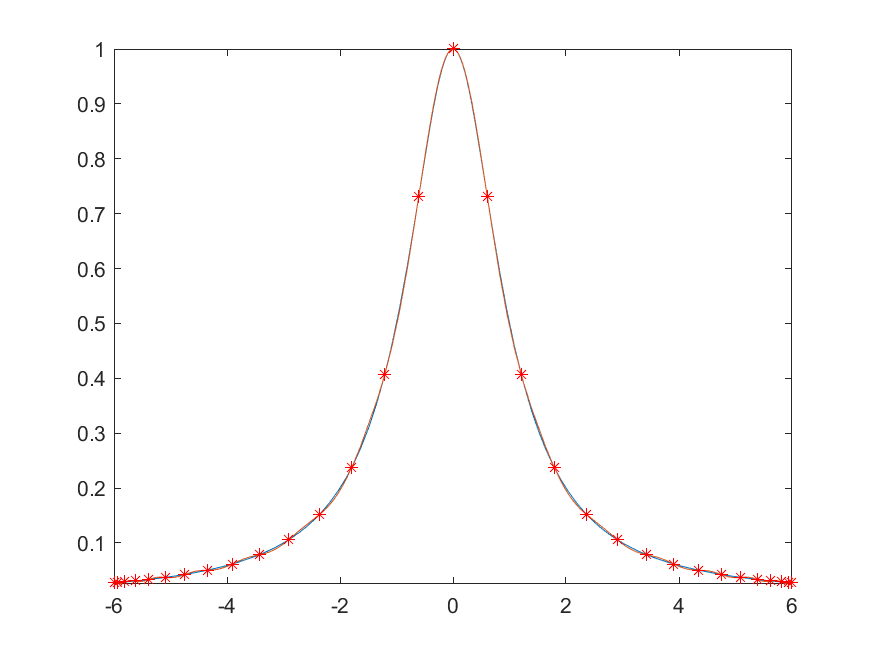
\includegraphics[scale=0.5]{cap4/4_7/30.png} &  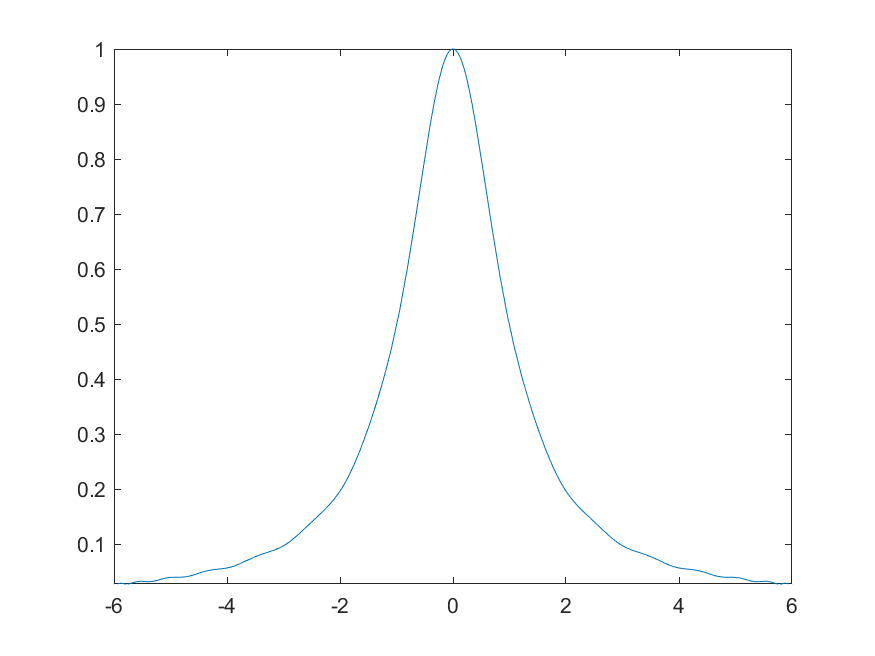
\includegraphics[scale=0.5]{cap4/4_7/32.png} \\

\hspace{3.5cm}\(n=34\) &  \(n=36\) \\
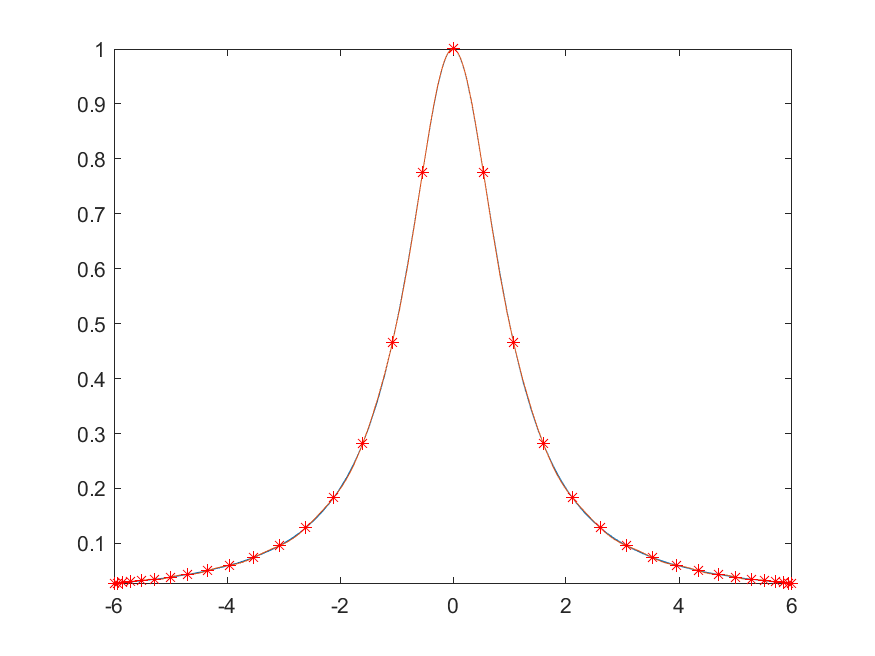
\includegraphics[scale=0.5]{cap4/4_7/34.png} &  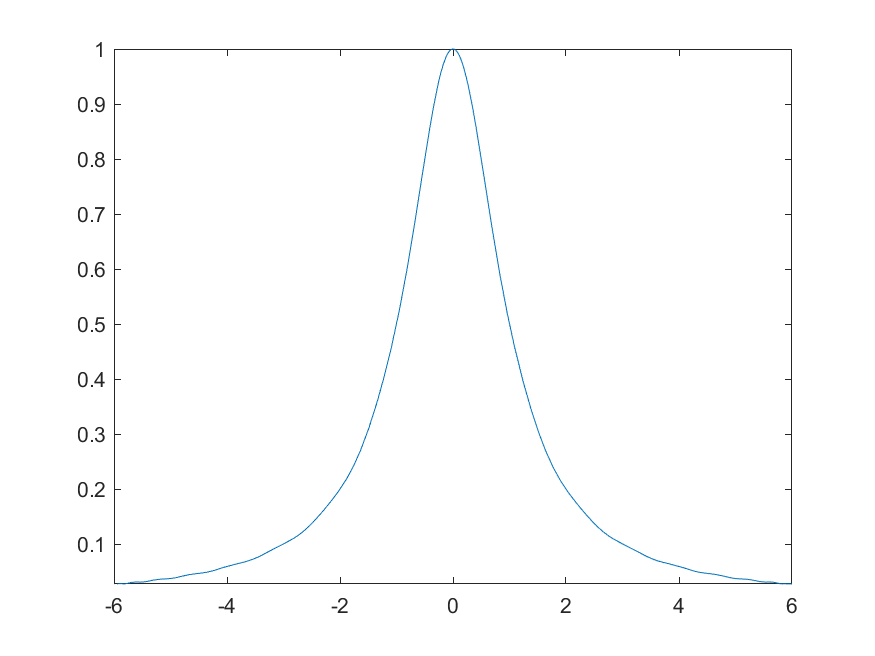
\includegraphics[scale=0.5]{cap4/4_7/36.png} \\

\hspace{3.5cm}\(n=38\) &  \(n=40\) \\
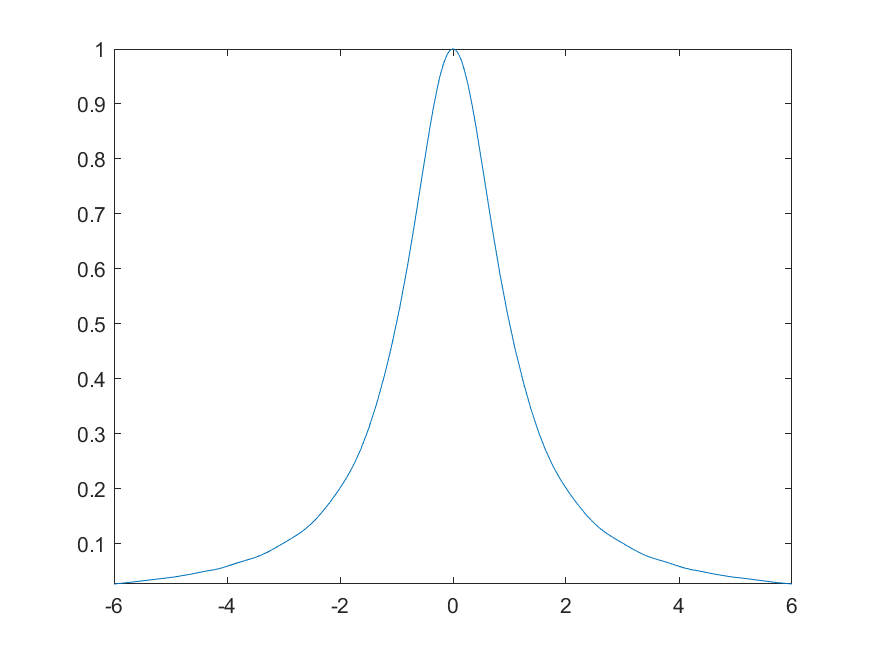
\includegraphics[scale=0.5]{cap4/4_7/38.png} &  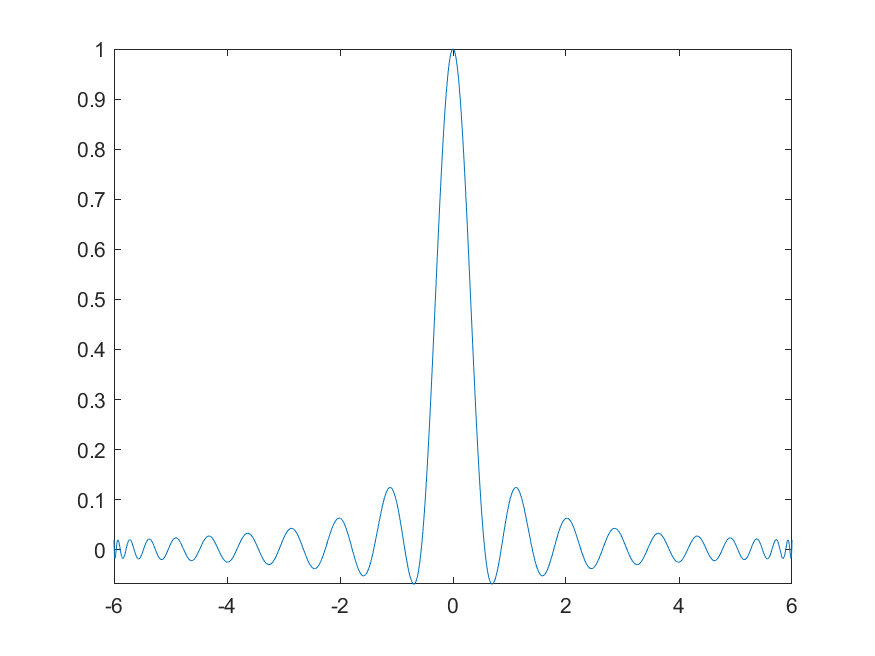
\includegraphics[scale=0.5]{cap4/4_7/40.png} \\
& \\
& \\
\end{tabular}


\noindent Riguardo all'errore commesso, grazie alla scelta dei nodi di Chebyshev come punti di interpolazione, per funzioni sufficientemente regolari abbiamo:
\[
||e|| \leq \frac{||f^{(n+1)}||}{(n+1)!2^n}
\]

\noindent Tuttavia, calcolare le derivate di ordine elevato della funzione di Runge risulterebbe molto dispendioso in termini computazionali. Quindi, ricaveremo una stima dell'errore in funzione di $n$ calcolandolo nel modo seguente:

$$
||e|| \approx ||f(x) - p_n(x)||_{\inf}
$$

\noindent con ovviamente $f$ intesa come la funzione di Runge e $p$ il suo polinomio interpolante.

\noindent L'errore così stimato è mostrato nella seguente tabella:

\begin{center}
	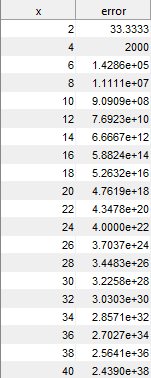
\includegraphics[scale=0.7]{cap4/4_7/4_7_error.png}
\end{center}

\noindent Come si pu\'o facilmente vedere, grazie alla scelta delle ascisse di Chebyshev come punti di interpolazione, l'errore diminuisce all'aumentare di \(n\), tendendo infatti a \(0\) per \(n \to \inf\).\\

\noindent Inoltre, \'e stato realizzato il seguente grafico mostrante l'andamento dell'errore nella parte destra dell'intervallo. La parte destra \'e stata omessa in quanto l'andamento dell'errore di interpolazione \'e simmetrico rispetto all'asse dellle ordinate: questo ha permesso di aumentare il livello di dettaglio del grafico, migliorandone la chiarezza e la visibilità.

\begin{center}
	\includegraphics[scale=0.7]{cap4/4_7/4_9_error.png}
\end{center}

\noindent Il codice Matlab con cui sono stati realizzati i grafci e la tabella mostrati sopra \'e il seguente: \\

\lstinputlisting[language=Matlab]{cap4/4_7.m}
